\chapter{Lentes gravitacionales}

\section{Consideraciones cosmológicas}

De acuerdo a la cosmología observacional, los modelos de mundo uniforme estándar pueden ser descritos por los siguientes parámetros \cite{2008gafo.book.....L}:\\

\textbf{La constante de Hubble} $H_0$ describe la razón de expansión presente del universo:

$$ H_0 = \left( \frac{\dot{a}}{a} \right)_{t_0} = \dot{a}(t_0),$$

\textbf{el parámetro de desaceleración} $q_0$ describe la desaceleración adimensional presente del universo:

$$ q_0 = -\left( \frac{\ddot{a} a }{\dot{a}^2} \right)_{t_0} = -\frac{\ddot{a}(t_0)}{H_0^2}, $$

y \textbf{el parámetro de densidad} $\Omega_0$ es la razón de la densidad de masa-energía presente del universo $\rho_0$ a la densidad crítica $\rho_c$:

$$\Omega_0 = \frac{\rho_0}{\rho_c} = \frac{8\pi G\rho_0}{3H_0^2}, $$

con $$ \rho_c = \frac{3H_0^2}{8\pi G}. $$

Otros parámetros útiles en términos de materia barionica y no barionica son:\\

y \textbf{El parámetro de densidad de los campos de vacío}, o la energía oscura:

\begin{eqnarray}
\Omega_{\Lambda} = \frac{8\pi G \rho_v}{3 H_0^2} = \frac{\Lambda}{3H_0^2},
\end{eqnarray}

con $\Lambda$ la cosntante cosmológica.\\

Éstos parámetros no son independientes, se tienen las siguientes dos ecuaciones:

$$ \kappa \left( \frac{c}{H_0} \right)^2 = (\Omega_0 + \Omega_{\Lambda}) - 1, $$

$$ q_0 = \frac{\Omega_0}{2} - \Omega_{\Lambda}. $$

La medida de distancias dependientes del \emph{redshift} son determinadas por la geometría y dinámica del Universo. Los parámetros $\Omega_{0} , \Omega_{\Lambda}$ pueden ser determinados directamente, pues si se conoce con precisión una distancia $D$ a un objeto por una técnica independiente del \emph{redshift}, se puede observar el comportamiento en gráficas como $D$ vs. $z$. Los parámetros cosmológicos también pueden ser probados por las propiedades de la materia oscura mediante técnicas de dinámica galáctica vista anteriormente y por el efecto de lentes gravitacionales como se detalla en este capítulo.\\

%La constante de Hubble es: $ H_0 = 70 \hspace{3mm} km s^{-1}  Mpc^{-1} $. 

Los parámetros cosmológicos son determinados por observaciones de objetos distantes tal como galaxias, cúmulos de galaxias y cuasares que son soportados por la Radiación cósmica de fondo de microondas  (CMB por sus siglas en inglés \emph{Cosmic Microwave Background Radiation}) y la distribución a gran escala de galaxias. Los siguientes valores para los parámetros cosmológicos son para un modelo plano $\Lambda$CDM con una ley de potencias simple del espectro de potencia (la constante de Hubble $H$ está reescalada en $h$ adimencional):

\begin{eqnarray}
 h &=& 0.73_{-0.03}^{+0.007} \\
 \omega_B = \Omega_B h^2 &=& 0.0223_{0.0009}^{0.0007} \\
  \omega_D = \Omega_D h^2 &=& 0.127_{0.0013}^{0.007}
\end{eqnarray}

con $\Omega_D$ el parámetro de densidad de materia oscura fría y  $\Omega_B$ el parámetro de densidad de Bariones. Para los cuales $\Omega_B + \Omega_D + \Omega_{\Lambda} +\Omega_k= 1$. Los datos son tomados de WMAP (Wilkinson Microwave Anisotropy Probe)\footnote{Ver: http://lambda.gsfc.nasa.gov/product/map/dr2/parameters\_info.cfm}.




\subsection{Distancia diametral angular}

Si un objeto tiene tamaño propio $L$, la luz toma un intervalo $\delta t$ y de la condición $ds = 0 (dr = s\theta = 0)$ se tiene que:

$$c \delta t = R(t_1) r \delta $$ 

con $t_1$ el tiempo de emisión y $\delta$ la separación angular , la distancia diametral angular está definida por:

$$ d_A = R(t_1) r $$

\begin{figure}
\centering%
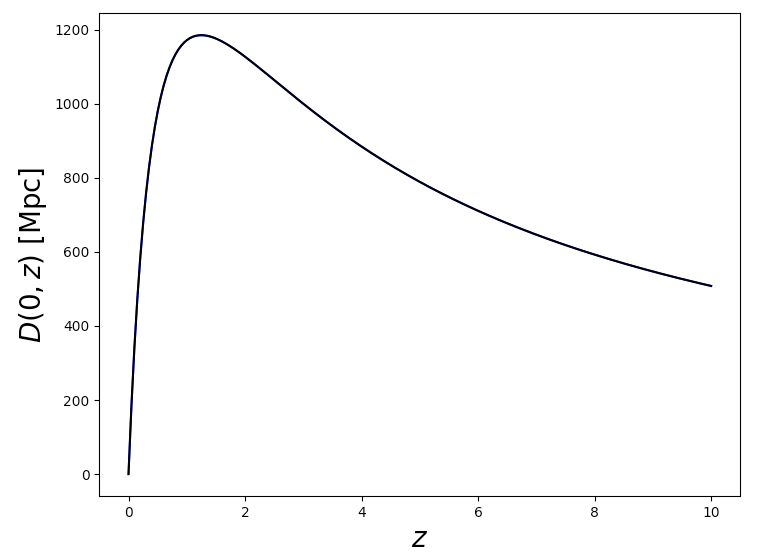
\includegraphics[width=0.9\columnwidth]{Kap3/d_A.png}%
\caption{Relación de la distancia diametral respecto a \emph{redshift}.}
\label{fig:grav_lens_1}
\end{figure}

La distancia diametral angular es función del \emph{redshift} $z$. En el caso de un universo plano se tiene \cite{CA10}:

\begin{equation}
D(0, z_s) = \frac{c}{H_0 (1+z_s)} = \int_0^{z_s} \frac{dz}{(1+z)\sqrt{\Omega_{mo}(1+z) + \Omega_{R0}(1+z)^2 +\Omega_{Q0}(1+z)^3 +\Omega_{k0} }}.
\end{equation}

La ecuación diferencial que relaciona la distancia $r$ a una fuente con \emph{redshift, z} está dada por:

\begin{eqnarray}
\left [  \Omega_{m0}z + 1 + \Omega_{Q0}(1+z)^{m-2} \left ( 1-\frac{1}{(1+z)^{m-2} } \right ) \right ] \frac{d^2 r}{d z^2} &+& \\
\frac{1}{1+z} \left [ \frac{7 \Omega_{m0}z }{2} + \frac{\Omega_{m0}}{2} + 3 + \Omega_{Q0} (1+z)^{m-2} \left ( \frac{m+4}{2} - \frac{3}{(1+z)^{m-2}} \right ) \right ] \frac{d r}{d z} &+& \\
\frac{3}{2(1+z)^4} \left [ \vec{\alpha} \Omega_{m0} (1+z)^3 + \vec{\alpha}_x \frac{m}{3} \Omega_{Q0} (1+z)^m \right ] r &=& 0
\end{eqnarray}

con condiciones de frontera dadas por:

\begin{eqnarray}
r(\textrm{z}_0, z_0) &=& 0 \\
\frac{dr \textrm{z}_0, z}{d z} |_{z = z_0} &=& H_0 \frac{dr_p(z_0)}{d z} |_{z = z_0} \\
    & = & \frac{1}{(1+z_0)^2 \sqrt{\Omega_{m0}z_0 + 1 + \Omega_{Q0}(1+z)^{m-2} \left [ 1-\frac{1}{(1+z_0)^{m-2} } \right ]  }}
\end{eqnarray}

%\cite{HU14}

\section{La ecuación de lente}

La ecuación de lente es la relación entre la posición angular de una fuente no afectada por el efecto de lente gravitacional, y la posición de sus imágenes si los rayos de luz que emanan de la fuente son perturbados por el campo gravitacional.\\

La masa total de un sistema estelar o de un cúmulo de galaxias puede ser encontrado a través del formalismo desarrollado como si ésta masa se comportara como lente gravitacional, donde el potencial gravitacional $\Psi$ correspondiente a la lente \emph{M} describe la deflexión  de los rayos de luz desde una fuente \emph{S} (tomado como una galaxia) hasta un observador \emph{O}, como se muestra en la Figura (\ref{fig:grav_lens_1}).\\

\begin{figure}
\centering%
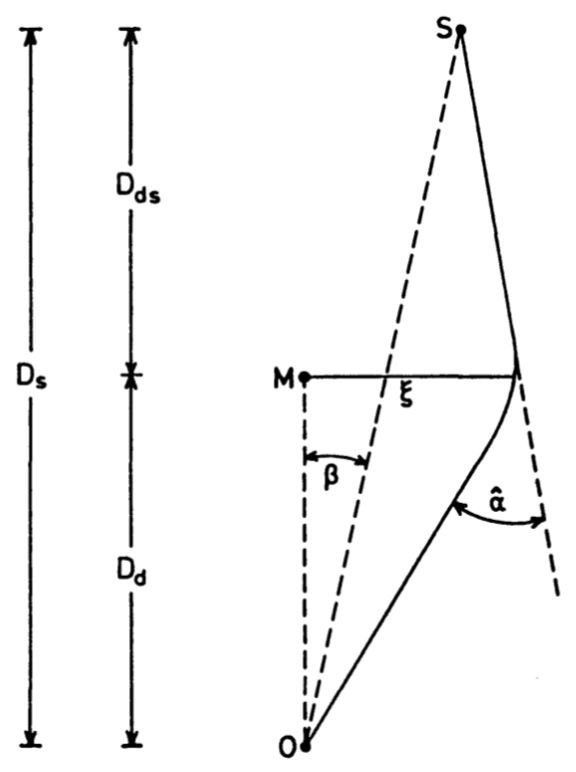
\includegraphics[width=0.4\columnwidth]{Kap3/grav_lens_1.png}%
\caption{Esquema de lente gravitacional \cite{SN92}.}
\label{fig:grav_lens_1}
\end{figure}

Las distancias diametrales angulares observador-lente $D_d$, observador-fuente $D_s$ y lente-fuente $D_{ds}$ relacionan el potencial de deflexión proyectado a lo largo de la línea de visión:

\begin{equation}
\Psi ( \bm{\theta}) = \frac{D_{ds}}{D_{d} D_{s}} \frac{2}{c^2} \int \Phi ( \bm{r} = D_d \bm{\theta}, z) dz,
\end{equation}

con los vectores de dos dimensiones $\bm{\theta} \equiv (x', y')$ en el plano del cielo, y $\bm{\beta} \equiv (x_s', y_s')$ dado por la relación vectorial:

\begin{equation}
\bm{\beta} = \bm{\theta}_i - \nabla_{\theta} \Psi (\bm{\theta}) |_{\bm{\theta}_i}
\end{equation}


La masa del sistema estelar, encerrada en el radio de Einstein $R_{ein}$ está dada por:

\begin{equation}
M_{ein} \equiv M(<R_{ein}) = \pi \Sigma_{crit}R_{ein}^2
\end{equation}

donde la densidad crítica $\Sigma_{crit}$ es la densidad de masa que ...

\begin{equation}
\Sigma_{crit} \equiv \frac{c^2}{4 \pi G} \frac{D_s}{D_d D_{ds}}
\end{equation}


\section{Modelos de lente}

\subsection{Modelos libres de escala}

Los modelos libres de escala con ley de potencias, con una disminución arbitraria en la parte exterior de la curva de rotación, tienen la característica que sus isofotas tienen la misma forma en cada radio y están completamente descritas por una función de forma $G(\theta)$. Ésta función depende solo del ángulo de posición $\theta$ con respecto al eje mayor. Esta descripción permite expresar el potencial de deflexión de la luz $\phi$ y la convergencia $\kappa$ proporcionales a $r$:

\begin{eqnarray}
\kappa &=& \frac{1}{2} G(\theta) r{\beta-2}, \\
\phi &=& r^{\beta} F(\theta)
\end{eqnarray}

en el plano de la lente. La potencia $\beta$ está restringida a $0<\beta<2$ para modelos galácticos , siendo $\beta=1$ en caso de una curva de rotación plana.\\

Bajo este modelo la función de forma $G(\theta)$ puede ser escrita como:

\begin{equation}
\label{G_theta}
G(\theta) = \beta^2 F(\theta) + F''(\theta), 
\end{equation}

donde dada una función $G(\theta)$ se puede hallar $F(\theta)$ solucionando la ecuación diferencial. Esto permite encontrar el potencial libre de escala correspondiente a un conjunto de contornos de igual densidad libres de escala \cite{EV03}.


\subsubsection{Método de expansión en serie de Fourier}

Las funciones $F(\theta), G(\theta)$ son periódicas, entonces se pueden expandir en serie de Fourier. Entonces expandiendo la función $F(\theta)$ y usando la ecuación (\ref{G_theta}):

\begin{eqnarray}
\label{Fourier_F}
F(\theta) &=& \frac{a_0}{2} + \sum_{k=1}^{\infty} \left[ a_k cos(k \theta) + b_k sin (k \theta) \right],\\
G(\theta) &=& \frac{a_0 \beta^2}{2} + \sum_{k=1}^{\infty} \left[ a_k (\beta^2-k^2) cos(k \theta) + b_k (\beta^2-k^2) sin (k \theta) \right],
\end{eqnarray}

Los coeficientes en la serie de Fourier debe satisfacer la condición $G(\theta) \geq 0$ para todo $\theta$ y obtener la densidad superficial positiva. 

\subsubsection{Las posiciones de las imágenes y los flujos}

Usando coordenadas polares en el plano de la imagen, la ecuación de lente tiene la forma:

\begin{eqnarray}
\xi & = & x - \frac{\partial \phi}{\partial x}, \\
\eta & = &  y - \frac{\partial \phi}{\partial y}
\end{eqnarray}



\begin{eqnarray}
\label{lens_equation_power_law}
\xi & = & r cos(\theta) - r^{\beta-1}\left[ \beta cos(\theta)F(\theta) - sin(\theta) F'(\theta)  \right] , \\
\eta & = &  r sin(\theta) - r^{\beta-1}\left[ \beta sin(\theta)F(\theta) - cos(\theta) F'(\theta)  \right]
\end{eqnarray}

donde $F(\theta)$ y $F'(\theta)$ están dadas por la serie de Fourier (\ref{Fourier_F}).\\

\subsubsection{Ajuste al modelo}

A continuación se describe el procedimiento para encontrar el valor de la potencia $\beta$, y una vez obtenido, la ecuación resultante es lineal y puede ser resuelta por métodos numéricos para la posición $(\xi, \eta)$ y los parámetros de Fourier $(a_k, b_k)$ dada una imagen observada en la posición

\begin{eqnarray}
x_i' &=& R_i' cos (\theta_i'),\\
y_i' &=& R_i' sin (\theta_i').
\end{eqnarray}
 
Se requiere minimizar la distancia entre \textbf{$\theta_{0i}$} y el modelo de lente predicho \textbf{$\theta_{pi}$} Para evitar resolver la ecuación de lente (\ref{lens_equation_power_law}) para  \textbf{$\theta_{pi}$}, se usa el tensor de magnificación para aproximar 

 

$$\bm{\theta} \approx \frac{\partial \bm{\theta}}{\partial \bm{\beta} } \bm{\beta} =  \bm{M} \bm{\beta},  $$

así entonces el modelo de mejor ajuste es tal que minimiza \cite{TR16} la cantidad

\[
\chi_{lens}^2 = \sum_{i} \left |
\begin{bmatrix}
    1/\Delta x & 0 \\
    0 & 1/\Delta y
\end{bmatrix}
\left ( \bm{\theta}_{pi} - \bm{\theta}_{0i} \right ) \right |^2 \approx \sum_{i} \left |
\begin{bmatrix}
    1/\Delta x & 0 \\
    0 & 1/\Delta y
\end{bmatrix}
 \bm{M}|_{\bm{\theta} = \bm{\theta}_{0i}} 
\begin{bmatrix}
    \xi_s' - \overline{\xi_s'} \\
    \eta_s' - \overline{\eta_s'}
\end{bmatrix}
 \right |^2 ,
\]

donde $(\Delta x, \Delta y)$ son los errores de medición de las posiciones $\bm{\theta}_{0i}$. Y $\bm{M}|_{\bm{\theta} = \bm{\theta}_{0i}}$ es el tensor de magnificación y $(\overline{\xi_s'}, \overline{\eta_s'})$ la posición de la fuente de acuerdo a la posición de la lente. \\

Por lo tanto la cantidad a minimizar es \cite{TR16}:

\begin{equation}
\chi^2 = \chi_{lens}^2 + \chi_{shape}^2,
\end{equation}

con $\chi_{shape}^2$ un término para restringir la forma de la distribución de masa a una elipse. Para encontrar la potencia $\beta$ se necesitan las razones de flujos para las imágenes.\\

En \cite{TR16} se encontró el modelo de lente como el mejor ajuste a las posiciones de lente de la imagen siguiendo el modelo libre de escala. En la figura \ref{fig:lens_model} se ilustra el resultado.

\begin{figure}
\centering%
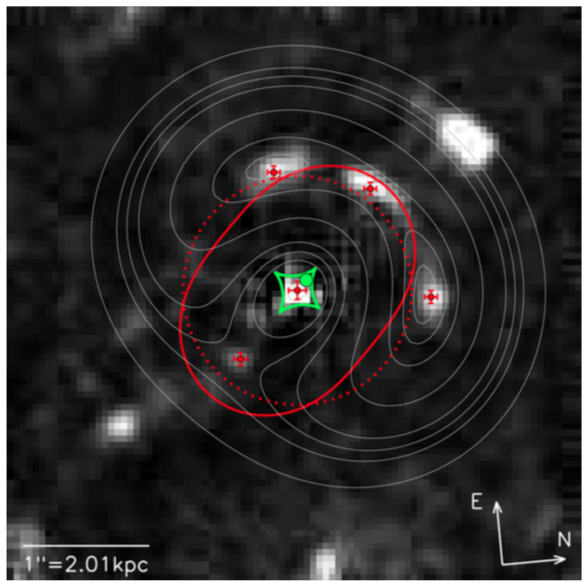
\includegraphics[width=0.8\columnwidth]{Kap3/lens_model.png}%
\caption{Modelo de lente para la lente en el centro de la galaxia espiral SDSS J1331+3628. La línea roja punteada es el círculo en el radio de Einstein, en la línea sólida roja se muestra la curva crítica y la caustica en la línea verde (tomado de \cite{TR16})}
\label{fig:lens_model}
\end{figure}


\begin{equation}
-----------------------------
\end{equation}




